\section{Multicast DNS LAB}
Solutions in this sections based on specification \href{https://tools.ietf.org/html/rfc6762}{RFC-6762}.

\subsection{}
The packets were sent to the IPv4 address 224.0.0.251, this IPv4 address is reserved for
mDNS, which  means a host can't have it.
\begin{center}
    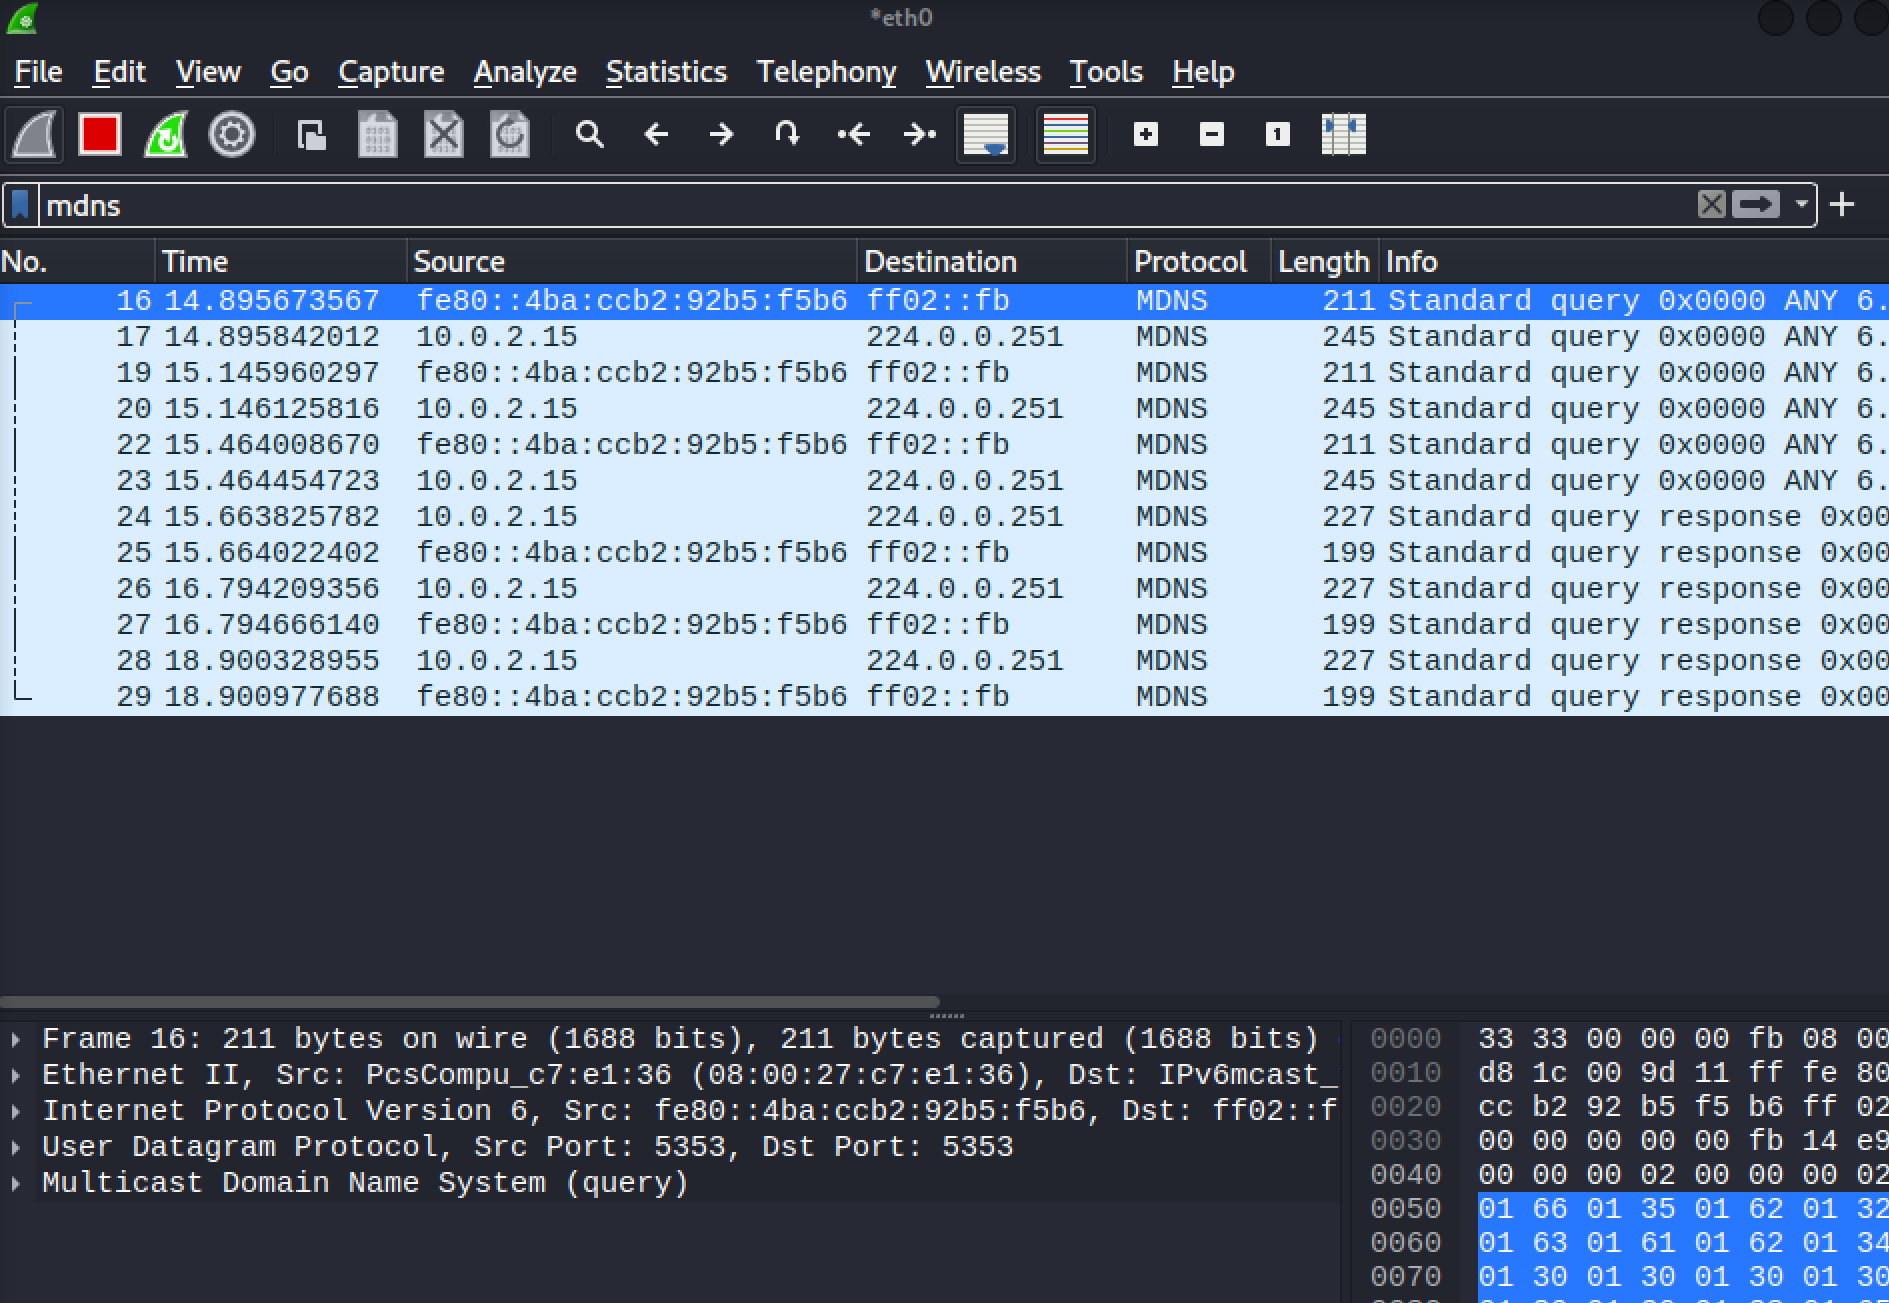
\includegraphics[width=1.2 \textwidth]{resources/q2-1.png}\centering
\end{center}


\subsection{}
\begin{itemize}
    \item \textbf{Advantage}: Other hosts now know and can cache the MDNS to IP mapping
    so that when they require it - they do not need to request for it; moreover - 
    they will be able to answer queries of others regarding the same hostname.
    \item \textbf{Disadvantage}: Sending the response using brodcast can and will cause
    un-nessecery traffic since it will often send the response packets to hosts that already know
    the mapping or ones that otherwise will not make use of it.
\end{itemize}

\subsection{}

The main resone we can think of is that brodcast generally
cannot be sent outside of the same LAN
\footnote{brodcast is generally not possbile from outside networks
since enabling it would expose the reciving network to DOS attacks - hence it is
often disallowed at the firewall.}, as opposed to multicast
which can - so using brodcast would limit the avalibility of the MDNS network
to just one LAN, or would require solving futher issues that would come with using
brodcast in remote networks.


\subsection{}
There are generally 3 options for how the end users or their client
applications might be able to know the addresses of internet devices.
\begin{enumerate}
    \item Standard DNS.
    \item Manually seaching for the IP address allocated by DHCP.
    \item Using MDNS.
\end{enumerate}
\textbf{Option 1} would not be practical for the purpose of IOT devices,
as it would require each such device to have it's own hostname at the global
DNS (which would be very expensive) - or would cause the user to manually configure
a local DNS service which is not a resonable request from the end user.\\

Similarly - \textbf{Option 2} also requires manual configuration and knowladge that the
end user does not have to implement.\\

Hence the best option we are left with is \textbf{Option 3} (MDNS) - which enables 'Plug and Play'
usage of the IOT devices.
